\chapter{DL4J}
\label{chap:java_dl4j}

\section{DL4J介绍}

Deeplearning4j(简称DL4J)是为Java和Scala编写的首个商业级开源分布式深度学习库。
DL4J还可与Hadoop和Spark集成,为商业化提供了很好的支持,而不仅仅是学术研究工具。
而在使用Deep Learning之前,我们还要先确定问题的类型,是有监督学习还是无监督问题?
对于有监督学习,你需要先提供有标签的数据进行训练;对于无监督学习,需要能自主检测数据的相似性和异常状况。

还要考虑处理的特征数量有多少?特征数量越多,需要的内存也越大。就图像而言,第一层的特征数量等于图像所包含的像素数。
所以MNIST数据集中的28 x 28像素的图像有784个特征。医疗诊断中的图像则可能有14兆像素。

\ \\
\begin{figure}[!htb]
\centerline{
\includegraphics{images/dl4j_logo.png}}
\label{fig:part3_dl4j_logo}
\end{figure}

主流的深度学习框架有TensorFlow、Caffe、Keras、Theano等,它们大多在单节点服务器通过GPU加速完成模型训练。
随着大数据时代的来临,使用分布式计算极大提高了计算性能。因此将分布式计算与深度学习结合成为必然趋势。
DL4J就是为此而生,利用Spark在多服务器多GPU上进行分布式的深度学习模型训练,让模型跑得更快。
运用DL4J高效的训练一个完整神经网络模型包括:
\begin{itemize}
\item[1.] 预加载数据,对数据进行预处理。DL4J提供了\emph{DataVec}简化数据采集过程。
\item[2.] 超参数配置,各种优化算法和学习率、激活函数等。
\item[3.] 构建神经网络,从单层到多层神经网络的构建。
\item[4.] 模型训练,借助ND4J和分布式计算,高效地训练模型。
\item[5.] 模型评估和保存。这正是DL4J的核心算法部分。
\end{itemize}

所以,在开始训练之前,要先花点时间学习如何使用DL4J的构建神经网络以及加载数据。
由于加载数据的过程(reshape、正则化、归一化等)很容易引入意想不到的错误,
DL4J提供了\emph{DataVec}类对数据加工预处理,不仅可以减少错误,还支持多种数据源,譬如图片、CSV、ARFF和纯文本等。

\section{构造网络}
DL4J的神经网络都是用NeuralNetConfiguration构建的,用它可以设定网络的层(layer)以及超参数。
典型的神经网络包含:输入和输出层,以及隐藏层。对于全连接层,在DL4J中也称为\emph{DenseLayer}。

\begin{figure}[!htb]
\centerline{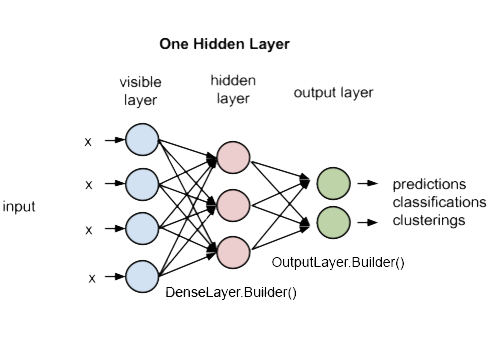
\includegraphics[width=.35\figwidth]{images/onelayer_labeled.png}}
\label{fig:part3_dl4j_onelayer}
\end{figure}


1. 设置超参数
\begin{lstlisting}[language=Java]
MultiLayerConfiguration conf = new NeuralNetConfiguration.Builder()
            .seed(rngSeed)
            .optimizationAlgo(OptimizationAlgorithm.STOCHASTIC_GRADIENT_DESCENT)
            .iterations(1)
            .learningRate(0.006)
            .updater(Updater.NESTEROVS).momentum(0.9)
            .regularization(true).l2(1e-4)
            .list()
\end{lstlisting}
\emph{超参数}(Hyperparameter)决定了神经网络学习方式的变量,包括模型的权重、激活函数、学习率和优化算法等。
\vspace{0.3cm}

2. 构建神经网络层
\begin{lstlisting}[language=Java]
.layer(0, new DenseLayer.Builder()
            .nIn(numRows * numColumns) // Number of input datapoints.
            .nOut(1000) // Number of output datapoints.
            .activation("relu") // Activation function.
            .weightInit(WeightInit.XAVIER) // Weight initialization.
            .build())
.layer(1, new OutputLayer.Builder(LossFunction.NEGATIVELOGLIKELIHOOD)
            .nIn(1000)
            .nOut(outputNum)
            .activation("softmax")
            .weightInit(WeightInit.XAVIER)
            .build())
.pretrain(false).backprop(true)
.build();
\end{lstlisting}

而\emph{超参数}(Hyperparameter)决定了神经网络学习方式的变量,包括模型的权重、激活函数、学习率和优化算法等。



\section{准备数据}
再好的训练模型,如果没有数据支撑,得出的结果也不是你想要的。本节将详细介绍常规数据使用方法,以及规范化手段。

\subsection{MNIST数据集}
MNIST(Mixed National Institute of Standards and Technology database)
是一个计算机视觉数据集,包含60000张手写数字的灰度图片训练集(training set) ,以及10000图片测试集(test set) 。
由来自250个不同人手写的数字构成,其中 50\% 是高中学生, 50\% 来自人口普查局 (the Census Bureau) 的工作人员。
测试集也是同样比例的手写数字数据。其中每一张图片都包含 $28 \times 28$ 个像素点,并配有对应的标签,也即是图片对应的数字。
\vspace{0.6cm}

\noindent
\figref{fig:part3_mnist_dataset},展示了测试集的组织形式:

\begin{figure}[!htb]
\centerline{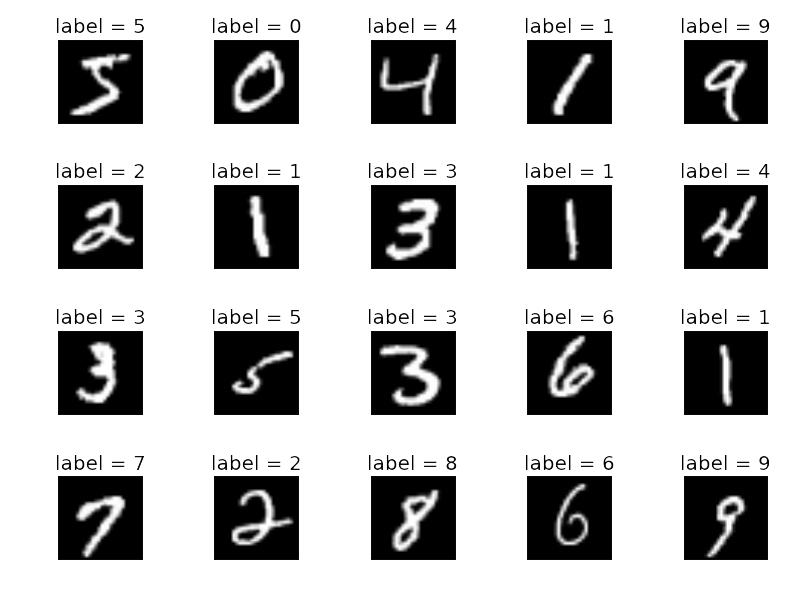
\includegraphics[width=.35\figwidth]{images/MNIST-dataset.png}}
\caption{MNIST数据}
\label{fig:part3_mnist_dataset}
\end{figure}

\noindent
MNIST官网提供了以下4个下载链接:
\begin{itemize}
\item[1.] train-images-idx3-ubyte.gz:  training set images (9912422 bytes) 
\item[2.] train-labels-idx1-ubyte.gz:  training set labels (28881 bytes) 
\item[3.] t10k-images-idx3-ubyte.gz:   test set images (1648877 bytes) 
\item[4.] t10k-labels-idx1-ubyte.gz:   test set labels (4542 bytes)
\end{itemize}

\noindent
看到这里,大家最更关心的还是下载的MNIST数据集,是如何定义的。这可以在官网查到,格式如下:
\vspace{0.3cm}

\noindent \textbf{训练集标签文件(train-labels-idx1-ubyte):}
\begin{lstlisting}
[偏移]    [数据类型]             [值]              [描述] 
0000       32 bit integer       0x00000801(2049)     magic number (MSB first) 
0004       32 bit integer       60000                number of items 
0008       unsigned byte        ??                   label 
0009       unsigned byte        ??                   label 
........ 
xxxx       unsigned byte        ??                   label
标签的值:0 ~ 9

16进制数据: 训练集-标签集合
0000 0801 0000 ea60 0500 0401 0902 0103
0104 0305 0306 0107 0208 0609 0400 0901
0102 0403 0207 0308 0609 0005 0600 0706
.....
\end{lstlisting}

\noindent \textbf{训练集数据文件(train-images-idx3-ubyte):}
\begin{lstlisting}
[偏移]     [数据类型]             [值]             [描述] 
0000       32 bit integer       0x00000803(2051)     magic number 
0004       32 bit integer       60000                number of images 
0008       32 bit integer       28                   number of rows 
0012       32 bit integer       28                   number of columns 
0016       unsigned byte        ??                   pixel 
0017       unsigned byte        ??                   pixel 
........ 
xxxx       unsigned byte        ??                   pixel

16进制数据: 训练集-图片集合
0000 0803 0000 ea60 0000 001c 0000 001c
0000 0000 0000 0000 0000 0000 0000 0000
.....
0000 0000 0000 0000 0000 0000 0000 0000
0000 0000 0000 0000 0312 1212 7e88 af1a
a6ff f77f 0000 0000 0000 0000 0000 0000
1e24 5e9a aafd fdfd fdfd e1ac fdf2 c340
.....
\end{lstlisting}

DL4J对MNIST数据集支持得很好,提供有deeplearning4j-datasets-xxxx.jar,其中有很多便利的API接口。



\subsection{IRIS数据集}
Iris也称鸢尾花卉数据集,是常用的分类实验数据集,由Fisher, 1936收集整理。包含150个数据集,分为3类,每类50个数据,每个数据包含4个属性。
可通过花萼长度,花萼宽度,花瓣长度,花瓣宽度4个属性预测鸢尾花卉属于(Setosa,Versicolour,Virginica)三个种类中的哪一类。

\begin{figure}[!htb]
\centerline{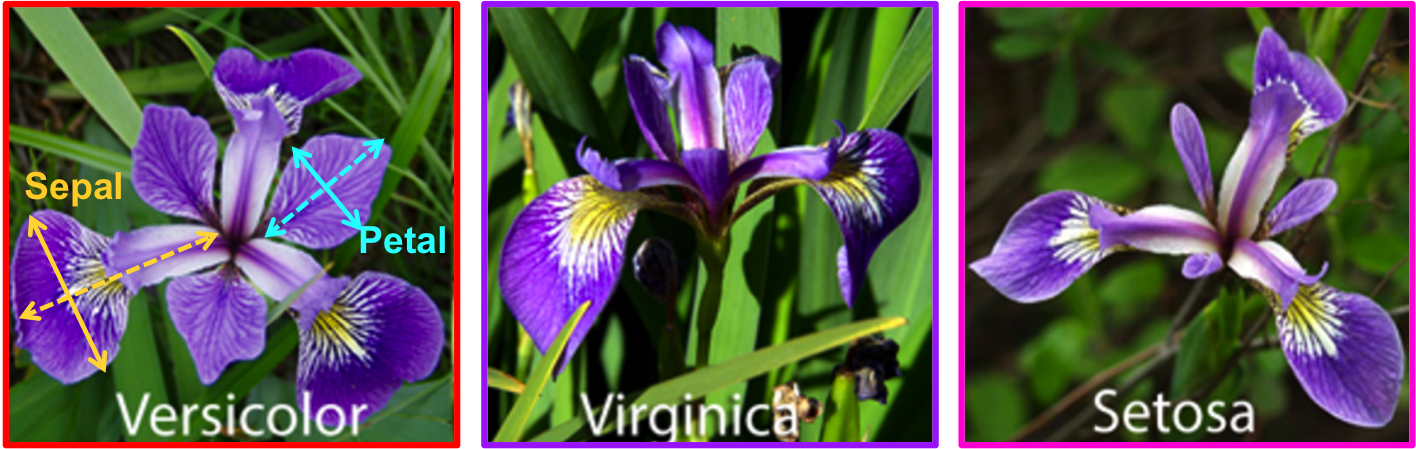
\includegraphics[width=.4\figwidth]{images/iris.png}}
\label{fig:part3_iris_flower}
\caption{莺尾花}
\end{figure}

该数据集由3种不同类型的鸢尾花的50个样本数据构成。其中的一个种类与另外两个种类是线性可分离的,后两个种类是非线性可分离的。
Iris以鸢尾花的特征作为数据来源,常用在分类操作中。该数据集包含了5个属性:

\begin{itemize}
\item[1.] Sepal.Length(花萼长度),单位是cm;
\item[2.] Sepal.Width(花萼宽度),单位是cm;
\item[3.] Petal.Length(花瓣长度),单位是cm;
\item[4.] Petal.Width(花瓣宽度),单位是cm;
\item[5.] 种类:Iris Setosa(山鸢尾)、Iris Versicolour(杂色鸢尾),以及Iris Virginica(维吉尼亚鸢尾)。
\end{itemize}


\subsection{波斯顿房价数据集}
波士顿房价数据集(Boston House Price Dataset)
,该数据集是美国人口普查局收集的有关波士顿马萨诸塞州住房的信息,发表于1978年美国某经济学杂志。
该数据集包含波士顿房屋的价格及其各项数据,每个数据项有14个数据,常用于回归分析。
\begin{itemize}
\item CRIM    - 城镇人均犯罪率
\item ZN      - 占地面积超过25,000平方英尺的住宅用地比例。
\item INDUS   - 城镇非零售商用土地的比例。
\item CHAS    - Charles River虚拟变量(如果是河道,则为1;否则为0)。
\item NOX     - 一氧化氮浓度(每千万)
\item RM      - 住宅平均房间数。
\item 年龄     - 1940年之前建成的自用房屋比例。
\item DIS     - 到波士顿五个中心区域的加权距离。
\item RAD     - 径向高速公路的可达性指数
\item 税       - 每10,000美元的全额物业税率
\item PTRATIO - 城镇的学生与教师比例
\item B       - $1000(Bk - 0.63)^ 2$,其中Bk是城镇黑人的比例
\item LSTAT   - 人口中地位低下者的比例。
\item MEDV    - 自有住房的中位数价值1000美元
\end{itemize}

波士顿房价数据集,共有506个观察,有13个输入变量和1个输出变量。在回归分析中,如果有两个或两个以上的自变量,就称为多元回归。
使用多个自变量的共同来预测,比只用一个自变量进行预测更符合实际,因此多元线性回归比一元线性回归的实用意义更大。
实际上,经常抽取波士顿房价数据的1-2个特征,做线性回归分析的演示。

\section{配置DL4J}
使用InteliJ IDEA开发环境,建议创建Maven工程,根据官网的说明配置pom.xml联网下载依赖就可以。
如果你比较熟悉Gradle,官网也有相应的说明。

\begin{lstlisting}[language=XML, caption={pom.xml}]
<dependencies>
  <dependency>
      <groupId>org.deeplearning4j</groupId>
      <artifactId>deeplearning4j-core</artifactId>
      <version>1.0.0-beta2</version>
  </dependency>
  <dependency>
      <groupId>org.nd4j</groupId>
      <artifactId>nd4j-native-plaform</artifactId>
      <version>1.0.0-beta2</version>
  </dependency>
</dependencies>
\end{lstlisting}


\section{线性回归}
线性回归可分为\emph{一元线性回归}和\emph{多元线性回归}。
只包括一个自变量和一个因变量的线性回归,结果近似一条直线。
\vspace{0.3cm}

\begin{tikzpicture}[scale=1.2]
    % Draw axes
    \draw [<->,thick] (0,2.5) node (yaxis) [above] {$y$}
        |- (4,0) node (xaxis) [right] {$x$};
    
    \draw (0,0.3) coordinate (a_1) -- (3,2.4) coordinate (a_2);

    \fill[red] (0.2,0.3) circle (2pt);
    \fill[red] (0.4,0.6) circle (2pt);
    \fill[red] (0.6,1.0) circle (2pt);

    \fill[red] (1.0,1.2) circle (2pt);
    \fill[red] (1.4,1.2) circle (2pt);
    \fill[red] (1.6,1.7) circle (2pt);

    \fill[red] (2.0,1.5) circle (2pt);
    \fill[red] (2.3,1.8) circle (2pt);

    \node[right=2.0cm, above=1.6cm] at (xaxis) {y=ax+b,其中x和y是已知的。};
    \node[right=2.0cm, above=0.6cm] at (xaxis) {求a=?,b=?};

    \draw[red,dashed] plot[smooth] coordinates {
        (0.2,0.3) (0.4,0.6) (0.6,1.0) (1.0,1.2)
        (1.4,1.2) (1.6,1.7) (2.0,1.5) (2.3,1.8)
    };

\end{tikzpicture}
\vspace{0.5cm}\noindent
上图,根据已知点如何预测下一个位置呢?若选用线性模型$y=a_n*x_n+a_{n-1}*x_{n-1}+\dots+a_0$可以拟合所有点,
但$y=a*x+b$简单的只是一条直线。选用哪个预测模型更好呢?更高维度的线性模型,实际上也就是多元线性回归:

\begin{equation}
y = \beta_0 + \beta_1x_1+\beta_2x_2+\dots+\beta_px_p+\epsilon
\end{equation}

\noindent
其中,$\epsilon$代表一些未知因素引入的随机误差(残差),譬如丢失一些关键特征。
这个误差会导致有些点偏离预测的函数曲线。在机器学习中,线性回归的模型描述通常使用$\hat{y}=w^Tx+b$的形式。
其中,$\hat{y}$是模型预测y应该取的值。

\begin{table}[!htbp]\centering
\begin{tabular}{|c|c|c|c|c|c|c|c|}
\hline
\multicolumn{8}{|c|}{已知数据}\\
\hline
1&2&3&4&5&6&7&8\\
\hline
(0.2,0.3)&(0.4,0.6)&(0.6,1.0)&(1.0,1.2)&(1.4,1.2)&(1.6,1.7)&(2.0,1.5)&(2.3,1.8)\\
\hline
\end{tabular}
\end{table}

对于简单的\emph{线性回归}问题,使用\emph{ND4J}和\emph{DL4J}都可以求解。
不同的是\emph{ND4J}结合最小二乘法直接公式求解,而\emph{DL4J}根据已知数据训练的结果。
\vspace{0.3cm}

1、创建神经网络
\begin{lstlisting}[language=Java]
OutputLayer outputLayer = new OutputLayer.Builder(LossFunctions.LossFunction.MSE)
                .activation(Activation.IDENTITY)
                .nIn(1)
                .nOut(1).build();

MultiLayerConfiguration conf = new NeuralNetConfiguration.Builder()
        .optimizationAlgo(OptimizationAlgorithm.STOCHASTIC_GRADIENT_DESCENT)
        .weightInit(WeightInit.ZERO)
        .updater(new Sgd(0.01))
        .list()
        .layer(0, outputLayer)
        .pretrain(false)
        .backprop(true).build();

MultiLayerNetwork net = new MultiLayerNetwork(conf);
net.init();
\end{lstlisting}

2、初始化数据
\begin{lstlisting}[language=Java]
double [] input = {
    0.2, 0.4, 0.6, 1.0, 1.4, 1.6, 2.0, 2.3
};

double [] output = {
    0.3, 0.6, 1.0, 1.2, 1.2, 1.7, 1.5, 1.8
};
INDArray inputNDArray = Nd4j.create(input, new int[]{input.length,1});
INDArray outPut = Nd4j.create(output, new int[]{output.length, 1});
\end{lstlisting}
3、机器学习过程
\begin{lstlisting}[language=Java]
for( int i=0; i<5000; i++ ) {
    net.fit(inputNDArray, outPut);
}

Map<String, INDArray> params = net.paramTable();
params.forEach((key, value) -> System.out.println("key:" + key +", value = " + value));
\end{lstlisting}

\begin{verbatim}
key:0_W, value = 0.6350
key:0_b, value = 0.4085
\end{verbatim}
\noindent
因此,拟合出的直线方程: $y=0.635*x+0.4085$

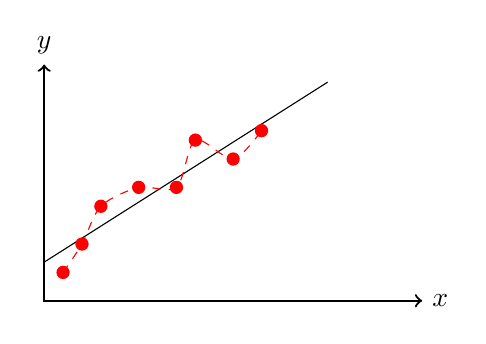
\begin{tikzpicture}[scale=1.2]
    % Draw axes
    \draw [<->,thick] (0,2.5) node (yaxis) [above] {$y$}
        |- (4,0) node (xaxis) [right] {$x$};
    
    \draw (0,0.4085) coordinate (a_1) -- (3,0.635*3+0.4085) coordinate (a_2);

    \fill[red] (0.2,0.3) circle (2pt);
    \fill[red] (0.4,0.6) circle (2pt);
    \fill[red] (0.6,1.0) circle (2pt);

    \fill[red] (1.0,1.2) circle (2pt);
    \fill[red] (1.4,1.2) circle (2pt);
    \fill[red] (1.6,1.7) circle (2pt);

    \fill[red] (2.0,1.5) circle (2pt);
    \fill[red] (2.3,1.8) circle (2pt);

    \draw[red,dashed] plot[smooth] coordinates {
        (0.2,0.3) (0.4,0.6) (0.6,1.0) (1.0,1.2)
        (1.4,1.2) (1.6,1.7) (2.0,1.5) (2.3,1.8)
    };

\end{tikzpicture}

\noindent
很显然,机器学习预测的图像,比上一页凭我直观的绘制直线更加符合实际。

\section{逻辑回归应用}
\section{多分类问题}
\section{聚类问题}
\section{卷积神经网络}
\section{循环卷积神经网络}







